%% ============================================================================
%% Artigo P2 PDI (versao em portugues) - template da disciplina
%% (template_pdi_com_tabelas_segmentacao.tex): Elsevier, Results in Engineering,
%% classe elsarticle, duas colunas (5p).
%% Tabelas em tables_pt/ geradas por scripts/08_artigo_pdi.py; figuras em figures_pt/.
%% Compilacao: latexmk -pdf main_pt.tex
%% ============================================================================
\documentclass[final,5p,times,twocolumn]{elsarticle}

%% Pacotes essenciais (template)
\usepackage[utf8]{inputenc}
\usepackage[T1]{fontenc}
\usepackage[brazil]{babel}
\usepackage{amsmath,amssymb,amsfonts}
\usepackage{icomma}
\usepackage{graphicx}
\usepackage{booktabs}
\usepackage{tabularx}
\usepackage{multirow}
\usepackage{array}
\usepackage{microtype}
\usepackage{lineno}
\usepackage[colorlinks=true,linkcolor=blue,citecolor=blue,urlcolor=blue]{hyperref}
%% Acrescimos deste artigo
\usepackage{tikz}
\usetikzlibrary{positioning,arrows.meta,calc,babel}

\biboptions{sort&compress}
\journal{Results in Engineering}
\modulolinenumbers[5]

\newcolumntype{L}[1]{>{\raggedright\arraybackslash}p{#1}}
\newcolumntype{Y}{>{\raggedright\arraybackslash}X}

\graphicspath{{figures_pt/}}
%% Posicionamento de floats: permite mais tabelas e figuras por pagina em duas colunas
\renewcommand{\topfraction}{0.9}
\renewcommand{\dbltopfraction}{0.9}
\renewcommand{\bottomfraction}{0.8}
\renewcommand{\textfraction}{0.07}
\renewcommand{\floatpagefraction}{0.75}
\renewcommand{\dblfloatpagefraction}{0.75}
\setcounter{topnumber}{4}
\setcounter{dbltopnumber}{4}
\setcounter{totalnumber}{6}
\newcommand{\ind}{\mathbf{1}}
%% Titulos do resumo e das palavras-chave em portugues (macros da classe elsarticle)
\abstracttitle{Resumo}
\keywordtitle{Palavras-chave}
\usepackage{etoolbox}
\makeatletter
\patchcmd{\printFirstPageNotes}{Email addresses:}{Endereços de e-mail:}{}{}
\patchcmd{\printFirstPageNotes}{Email address:}{Endereço de e-mail:}{}{}
\makeatother

\begin{document}

%% ============================================================================
%% CABECALHO (FRONTMATTER)
%% ============================================================================
\begin{frontmatter}

\title{Segmentação temporal das regiões de reação ativa no sistema de Gray-Scott do The Well: pré-processamento, arquiteturas e pós-processamento}

\author[a]{Andre Luis Aguiar do Nascimento}
\ead{andre.aguiar@discente.ufma.br}

\author[a]{Joao Guilherme Miranda Lago}
\ead{jglago10@gmail.com}

\author[a]{Wesley dos Santos Gatinho}
\ead{wesley.gatinho@discente.ufma.br}

\affiliation[a]{%
    organization={Universidade Federal do Maranh\~ao (UFMA)},
    city={S\~ao Lu\'is},
    postcode={65080-805},
    country={Brasil}
}

\begin{abstract}
Sistemas de reação-difusão descrevem reatores químicos, o espalhamento de substâncias que reagem entre si e a formação de padrões biológicos, e quantificar onde suas estruturas estão e como evoluem exige segmentar os campos de concentração ao longo do tempo. Este trabalho avalia como o pré-processamento, a arquitetura de segmentação e o pós-processamento afetam a segmentação das regiões de reação ativa no sistema bidimensional de Gray-Scott do The Well, sob um protocolo comum a uma turma de Processamento Digital de Imagens. A referência limiariza a espécie autocatalítica $B$ pelo método de Otsu em um instante intermediário da simulação, e as redes a recuperam a partir do substrato $A$ na resolução nativa de $128\times128$. Dez pré-processamentos, três arquiteturas (U-Net, SegFormer e Mask2Former, com 20 épocas de treino cada) e cinco pós-processamentos foram aplicados às 1.200 trajetórias, o que resultou nas 150 combinações da matriz do protocolo e em 48 linhas de \textit{baseline}. Em 120 trajetórias de teste, a U-Net obteve Dice de 0,953 sem pré e pós-processamento, contra 0,892 do SegFormer, 0,768 do Mask2Former e 0,888 da limiarização de Otsu em $A$. O pré-processamento alterou o Dice em no máximo 1,37 ponto percentual, e o filtro temporal o reduziu em 8,6 a 11,3 pontos. Os maiores ganhos vieram do instante inicial aleatório: excluído esse instante, a otimização do limiar reduziu o Dice da U-Net e do SegFormer. Nesse conjunto, a resolução de saída da arquitetura pesou mais que as técnicas aplicadas a seu redor, e a seleção de configurações pelo Dice médio mostrou-se sensível a um único quadro sem informação física.
\end{abstract}

\begin{keyword}
modelo de Gray-Scott \sep
reação-difusão \sep
segmentação semântica \sep
U-Net \sep
SegFormer \sep
Mask2Former \sep
The Well
\end{keyword}

\end{frontmatter}

%% ============================================================================
%% SUMARIO
%% ============================================================================
\setcounter{tocdepth}{2}
\tableofcontents
\vspace{1em}

%% ============================================================================
\section{Introdução}\label{sec:intro}

Sistemas de reação-difusão descrevem substâncias que se espalham no espaço enquanto reagem entre si. Quando as espécies difundem com velocidades diferentes, a difusão, que isoladamente suaviza qualquer perturbação, pode desestabilizar um meio homogêneo e dar origem a manchas, labirintos e ondas que surgem sem comando externo. Turing~\cite{turing1952} propôs esse mecanismo para explicar a morfogênese; o mesmo arcabouço foi usado para descrever padrões biológicos~\cite{kondo2010,murray2003} e foi observado experimentalmente em reatores químicos~\cite{lee1993}. O modelo de Gray-Scott é a forma mínima desse fenômeno: duas espécies, uma reação autocatalítica cúbica e dois parâmetros de controle bastam para gerar padrões estacionários e dinâmicos qualitativamente distintos~\cite{gray1983,pearson1993}. Analisar um padrão desse tipo exige responder onde estão as estruturas de interesse e como elas evoluem ao longo do tempo, isto é, segmentar o campo contínuo em regiões.

A coleção The Well disponibiliza simulações do sistema de Gray-Scott, entre outros sistemas físicos, para o desenvolvimento de métodos de aprendizado de máquina~\cite{ohana2024well}. Nessa coleção, os modelos de referência são substitutos neurais, como o Fourier Neural Operator, que preveem os próximos estados do campo~\cite{li2021fno,brunton2020}. A previsão, porém, não localiza as estruturas nem mede sua formação, migração ou extinção. A segmentação semântica por redes profundas, consolidada em imagens naturais e médicas~\cite{long2015fcn,ronneberger2015unet,xie2021segformer,cheng2022mask2former}, oferece essa representação, mas seu comportamento em campos simulados, sem textura, em domínio periódico e com estruturas que surgem e desaparecem, é menos documentado. Além disso, etapas clássicas que antecedem a rede, como normalizações e filtros, ou que a sucedem, como a limiarização e a morfologia, costumam ser aplicadas sem que se meça se e por que alteram a segmentação.

Nesse contexto, este trabalho avalia o efeito do pré-processamento, da arquitetura de segmentação e do pós-processamento sobre a segmentação temporal das regiões de reação ativa no sistema de Gray-Scott do The Well. O estudo segue um protocolo comum a uma turma de Processamento Digital de Imagens, no qual cada participante aplica o mesmo experimento a um conjunto bidimensional diferente: dez pré-processamentos, três arquiteturas e cinco pós-processamentos, entrada de no máximo 128 pixels no maior eixo sem ampliação, subconjunto de até 25~GB por conjunto e 20 épocas de treino. O experimento é organizado em quatro condições: a arquitetura sozinha, o pré-processamento seguido da arquitetura, a arquitetura seguida do pós-processamento e a combinação das três etapas. Quatro perguntas de pesquisa orientam o estudo: (PP1) como a U-Net, o SegFormer e o Mask2Former se comparam entre si e com uma referência sem aprendizado; (PP2) em que medida o pré-processamento altera a segmentação de cada arquitetura; (PP3) em que medida o pós-processamento a altera; e (PP4) se as máscaras acompanham a evolução temporal das estruturas, inclusive sua formação e sua extinção.

A contribuição é empírica e descritiva: uma referência definida por critério físico, a avaliação das 150 combinações do protocolo e de suas linhas de \textit{baseline} com métricas por classe, temporais e de custo, análises pareadas que isolam o efeito de cada técnica e uma análise de sensibilidade ao instante inicial. Não se propõe uma nova arquitetura. O alcance dos resultados é delimitado por uma única semente de aleatoriedade (\textit{seed}) por treino, por uma referência obtida por limiarização, e não por anotação especialista, e pela adaptação do treino do Mask2Former ao orçamento disponível (Seção~\ref{subsec:architectures}).

A Seção~\ref{sec:sec2} apresenta o sistema de Gray-Scott, suas aplicações e o conjunto de dados; as Seções~\ref{sec:sec3} a~\ref{sec:sec5} descrevem as arquiteturas, as técnicas de processamento e as métricas; a Seção~\ref{sec:experimental} apresenta o protocolo e os resultados, discutidos na Seção~\ref{sec:sec6}; e a Seção~\ref{sec:conclusions} conclui o trabalho.

%% ============================================================================
\section{O sistema de reação-difusão de Gray-Scott}\label{sec:sec2}

\subsection{Reação-difusão e o mecanismo de Turing}\label{subsec:turing}

Um sistema de reação-difusão com duas espécies de concentrações $u(\mathbf{x},t)$ e $v(\mathbf{x},t)$ é descrito por
\begin{equation}\label{eq:rd}
\frac{\partial u}{\partial t} = D_u \nabla^2 u + f(u,v), \qquad
\frac{\partial v}{\partial t} = D_v \nabla^2 v + g(u,v),
\end{equation}
em que $\nabla^2$ é o laplaciano, responsável pelo espalhamento espacial segundo a lei de Fick, e $f$ e $g$ representam a cinética local. Seja $(u^*,v^*)$ um estado homogêneo estacionário e $\mathbf{J}$ a matriz jacobiana da cinética nesse estado. Uma perturbação proporcional a $e^{\lambda t+i\mathbf{q}\cdot\mathbf{x}}$ cresce com a taxa dada pelos autovalores de $\mathbf{J}-q^2\mathbf{D}$, com $\mathbf{D}=\mathrm{diag}(D_u,D_v)$. Turing~\cite{turing1952} mostrou que um estado estável na ausência de difusão ($\operatorname{tr}\mathbf{J}<0$ e $\det\mathbf{J}>0$) pode ser desestabilizado por ela se
\begin{equation}\label{eq:turing}
h(q^2)=D_uD_v q^4-(D_u J_{22} + D_v J_{11})\,q^2+\det\mathbf{J} < 0
\end{equation}
para algum $q$, o que só ocorre quando as espécies difundem com velocidades suficientemente diferentes. A faixa de números de onda instáveis define o comprimento característico do padrão, independentemente do tamanho do domínio~\cite{murray2003}.

\subsection{O modelo de Gray-Scott}\label{subsec:gsmodel}

O modelo de Gray-Scott descreve um reator isotérmico alimentado continuamente, no qual um substrato $A$ é convertido pela etapa autocatalítica $A+2B\rightarrow 3B$ e o autocatalisador decai segundo $B\rightarrow P$, sendo $P$ um produto inerte~\cite{gray1983,gray1984}. Na forma adimensional e espacialmente estendida,
\begin{subequations}\label{eq:gs}
\begin{align}
\frac{\partial A}{\partial t} &= \delta_A\nabla^2 A - A B^2 + F\,(1-A), \label{eq:gsA}\\
\frac{\partial B}{\partial t} &= \delta_B\nabla^2 B + A B^2 - (F+k)\,B, \label{eq:gsB}
\end{align}
\end{subequations}
em que $AB^2$ é a taxa da reação, que consome $A$ e produz $B$, $F$ é a taxa de alimentação de $A$, e $k$ é a taxa de remoção de $B$. O estado trivial $(A,B)=(1,0)$ sempre existe e é linearmente estável, com autovalores $-F$ e $-(F+k)$; ele representa um reator no qual o autocatalisador desapareceu. Os estados não triviais satisfazem $AB=F+k$ e $F(1-A)=(F+k)B$, de modo que
\begin{equation}\label{eq:gsfixed}
B_\pm=\frac{F\pm\sqrt{F^2-4F(F+k)^2}}{2(F+k)},\qquad A_\pm=\frac{F+k}{B_\pm},
\end{equation}
que existem somente abaixo da curva de sela-nó $k=\tfrac12\sqrt{F}-F$ no plano $(F,k)$, com jacobiana
\begin{equation}\label{eq:gsjac}
\mathbf{J}=\begin{pmatrix} -B^{*2}-F & -2(F+k)\\ B^{*2} & F+k\end{pmatrix}.
\end{equation}
Pearson~\cite{pearson1993} mostrou que, próximo dessas fronteiras, perturbações localizadas do estado trivial evoluem para manchas autorreplicantes, pulsos que se deslocam e labirintos, conforme a região do plano $(F,k)$. Duas consequências importam para a segmentação: pequenas alterações de $(F,k)$ mudam qualitativamente o padrão, e, para alguns parâmetros, o padrão colapsa para o estado trivial, de modo que todas as estruturas desaparecem.

As Equações~\eqref{eq:gsA} e~\eqref{eq:gsB} também explicam a relação entre os dois campos usada neste estudo. Onde a reação está ativa, $B$ é elevado, e $A$ é consumido, o que torna os campos anticorrelacionados. Como $A$ difunde duas vezes mais rápido que $B$ nas simulações utilizadas, a região de depleção de $A$ em torno de uma estrutura é mais larga e mais suave que a própria estrutura. Por isso, a fronteira $\{B=\tau\}$ não coincide com uma isolinha de $A$, e recuperá-la a partir de $A$ constitui um problema inverso não linear e não local.

\subsection{Onde o sistema de Gray-Scott se aplica}\label{subsec:applications}

Na engenharia de reatores químicos, o modelo foi formulado para explicar multiestabilidade, ignição, extinção e oscilações em reatores contínuos com autocatálise cúbica~\cite{gray1983,gray1984}, e sua forma espacial descreve reatores de gel, nos quais as manchas autorreplicantes previstas foram observadas~\cite{lee1993}; a região $\{B>\tau\}$ corresponde, então, à região em que a reação está ativa, e sua área ao longo do tempo, inclusive seu colapso, relaciona-se ao rendimento do reator. Em segurança industrial, o planejamento de emergência simula o vazamento de um gás que se espalha enquanto reage com o ar para delimitar, a cada instante, a região em que a concentração ultrapassa um limiar, que é a operação estudada aqui. Na biologia, modelos de tipo Turing explicam padrões de pigmentação~\cite{kondo2010,murray2003}, e a segmentação converte o padrão em número, tamanho e espaçamento de estruturas. No aprendizado de máquina científico, a segmentação fornece um diagnóstico, em nível de estrutura, dos substitutos neurais avaliados no The Well~\cite{ohana2024well}.

\subsection{O conjunto \texttt{gray\_scott\_reaction\_diffusion}}\label{subsec:dataset}

O conjunto reúne 1.200 trajetórias: seis conjuntos de parâmetros, que correspondem a regimes de padrão, cada um com 200 condições iniciais aleatórias, divididas por trajetória em 160, 20 e 20 para treino, validação e teste~\cite{ohana2024well}. Os regimes são \textit{gliders}, \textit{bubbles}, \textit{maze}, \textit{worms}, \textit{spirals} e \textit{spots}, cujos parâmetros $(F,k)$ estão na Tabela~\ref{tab:regimes}. Todas as simulações usam $\delta_A=2\times10^{-5}$ e $\delta_B=10^{-5}$ no quadrado periódico $[-1,1]^2$ com $128\times128$ pontos, discretização pseudoespectral de Fourier e integração temporal por diferenças exponenciais de quarta ordem (ETDRK4)~\cite{cox2002,kassam2005}. Os instantes são armazenados a cada 10 unidades de tempo até $t=10.000$, o que resulta em 1.001 instantes por trajetória e 154~GB; aqui, o tempo é indexado pelo número do instante $n\in\{0,\dots,1000\}$. Diversas trajetórias do regime \textit{gliders} atingem um estado estacionário homogêneo, fato tratado na construção da referência.

%% ============================================================================
\section{Arquiteturas de segmentação}\label{sec:sec3}

A segmentação semântica atribui um rótulo a cada pixel, aqui fundo ou estrutura; as redes totalmente convolucionais a tornaram um problema de aprendizado de ponta a ponta~\cite{long2015fcn}, e as três arquiteturas avaliadas representam famílias de projeto distintas.

\subsection{U-Net}\label{subsec:unet}

A U-Net é um codificador-decodificador simétrico~\cite{ronneberger2015unet}. O codificador reduz progressivamente a resolução e aumenta o número de canais, e o decodificador recupera a resolução original. Em cada escala, uma conexão de salto concatena o mapa do decodificador ao mapa do codificador de mesma resolução, reintroduzindo detalhes espaciais perdidos na redução. Neste estudo, o codificador é uma ResNet-34 pré-treinada no ImageNet~\cite{he2016resnet,deng2009imagenet}, cujos blocos residuais calculam $\mathbf{y}=\mathcal{F}(\mathbf{x})+\mathbf{x}$, totalizando 24,4 milhões de parâmetros. A saída é um mapa de \textit{logits} $z$ na resolução de entrada, e a probabilidade de estrutura é $p=\sigma(z)$.

\subsection{SegFormer}\label{subsec:segformer}

Os Transformers substituem a convolução pela autoatenção, $\mathrm{Attn}(Q,K,V)=\mathrm{softmax}(QK^\top/\sqrt{d})\,V$, na qual cada \textit{token} interage com todos os demais~\cite{vaswani2017}; o Vision Transformer aplica essa operação a recortes da imagem~\cite{dosovitskiy2021vit}. O SegFormer adapta a ideia à predição densa com um codificador hierárquico, o Mix Transformer, inspirado no PVT~\cite{wang2021pvt,xie2021segformer}, que produz mapas em $1/4$, $1/8$, $1/16$ e $1/32$ da resolução de entrada. Seus componentes são a fusão sobreposta de recortes por convoluções com passo; a autoatenção eficiente, na qual chaves e valores são reduzidos espacialmente por uma razão $R$, o que reduz o custo de $O(N^2)$ para $O(N^2/R)$; a Mix-FFN, cuja convolução $3\times3$ fornece informação posicional sem codificação posicional explícita; e um decodificador formado apenas por camadas MLP, que projeta as quatro escalas, as amplia para $1/4$ da resolução e as funde. Foi usada a variante MiT-B2, pré-treinada no ImageNet-1k, com 27,3 milhões de parâmetros.

\subsection{Mask2Former}\label{subsec:mask2former}

O MaskFormer reformulou a segmentação como classificação de máscaras: em vez de classificar cada pixel, o modelo prevê um conjunto de $N$ pares $\{(p_i,m_i)\}_{i=1}^N$, cada um formado por uma distribuição $p_i$ sobre $K$ classes e uma classe ``sem objeto'' e por uma máscara binária $m_i$~\cite{cheng2021maskformer}, na linha do DETR~\cite{carion2020detr}. O Mask2Former combina um \textit{backbone}, aqui o Swin-T, com autoatenção em janelas deslocadas~\cite{liu2021swin}, um decodificador de pixels com atenção deformável em múltiplas escalas~\cite{zhu2021deformable} e um decodificador Transformer cujas $N$ consultas aprendíveis usam atenção mascarada~\cite{cheng2022mask2former},
\begin{equation}\label{eq:maskedattn}
\mathbf{X}_l=\mathrm{softmax}(\mathcal{M}_{l-1}+\mathbf{Q}_l\mathbf{K}_l^\top)\mathbf{V}_l+\mathbf{X}_{l-1},
\end{equation}
com $\mathcal{M}_{l-1}(x,y)=0$ onde $m_{l-1}(x,y)\geq 0,5$ e $-\infty$ nos demais pixels, de modo que cada consulta atende apenas à região de sua máscara corrente. No treino, as previsões são associadas uma a uma aos segmentos de referência pelo algoritmo húngaro~\cite{kuhn1955}, e a perda é $\mathcal{L}=\lambda_{ce}\mathcal{L}_{ce}+\lambda_{bce}\mathcal{L}_{bce}+\lambda_{dice}\mathcal{L}_{dice}$, com $\lambda=(2,5,5)$; na receita original, essa perda é aplicada também à saída de cada camada intermediária do decodificador, o que se denomina supervisão profunda. Na inferência semântica, o escore da classe $c$ em cada pixel é $\sum_i p_i(c)\,m_i(x,y)$. Foi usado o modelo Swin-T treinado no ADE20K~\cite{zhou2017ade}, com 47,4 milhões de parâmetros e $N=100$ consultas; seu classificador foi substituído por um de duas classes.

\subsection{Resolução de saída}\label{subsec:outres}

A U-Net prevê na resolução da entrada, enquanto o SegFormer e o Mask2Former preveem em $1/4$ dela. Para uma entrada de $128\times128$, a saída dessas duas arquiteturas tem $32\times32$ células e é interpolada bilinearmente para $128\times128$. Essa diferença é uma propriedade das arquiteturas e é retomada na Seção~\ref{sec:sec6}.

%% ============================================================================
\section{Pré-processamento e pós-processamento}\label{sec:sec4}

\subsection{Pré-processamento}\label{subsec:pretheory}

O pré-processamento modifica o campo antes da rede. As normalizações alteram os valores com estatísticas do treino: o \textit{z-score} calcula $x'=(x-\mu)/\sigma$; a normalização RMS divide pela raiz da média quadrática, $x'=x/\sqrt{\overline{x^2}}$, preservando o zero e a forma da distribuição; o escalonamento robusto calcula $x'=(x-\mathrm{med})/\mathrm{IIQ}$, pouco sensível a valores extremos; a normalização mín-máx calcula $x'=(x-x_{\min})/(x_{\max}-x_{\min})$; e o recorte por percentis satura os valores fora de $[p_1,p_{99}]$. Os filtros espaciais alteram a estrutura do campo~\cite{gonzalez2018}. A suavização gaussiana, $x'=G_\sigma * x$, multiplica o espectro por $e^{-\sigma^2q^2/2}$; o filtro de mediana substitui cada pixel pela mediana da vizinhança; o filtro bilateral pondera os vizinhos pela distância espacial e pela diferença de intensidade, suavizando regiões homogêneas e preservando bordas~\cite{tomasi1998}; a difusão anisotrópica de Perona-Malik resolve
\begin{equation}\label{eq:pm}
\partial_\tau I=\nabla\cdot\big(c(|\nabla I|)\nabla I\big),\qquad c(s)=e^{-(s/\kappa)^2},
\end{equation}
o que inibe a difusão através de gradientes fortes~\cite{perona1990}; e a remoção de ruído por \textit{wavelets} limiariza suavemente os coeficientes de detalhe, $\eta_\lambda(w)=\mathrm{sign}(w)\max(|w|-\lambda,0)$, com o limiar adaptativo BayesShrink $\lambda=\hat\sigma_n^2/\hat\sigma_x$~\cite{donoho1994,chang2000,daubechies1992}.

\subsection{Pós-processamento}\label{subsec:posttheory}

O pós-processamento converte o mapa de probabilidades $P(x,y)\in[0,1]$ na máscara final. A otimização do limiar escolhe $\tau$ em $\ind[P>\tau]$ para corrigir o viés de calibração da rede. A abertura morfológica, $\gamma_B(X)=(X\ominus B)\oplus B$, remove objetos menores que o elemento estruturante $B$, e o fechamento, $\varphi_B(X)=(X\oplus B)\ominus B$, preenche lacunas estreitas e reconecta partes próximas~\cite{serra1982,soille2003}. A filtragem de componentes conexos remove regiões cuja área é inferior a um mínimo, sob a hipótese de que componentes muito pequenos são ruído. A filtragem de consistência temporal aplica a mediana das probabilidades de $w$ instantes consecutivos de uma mesma trajetória antes da limiarização, reduzindo oscilações entre quadros.

%% ============================================================================
\section{Métricas de avaliação}\label{sec:sec5}

\subsection{Métricas de sobreposição e por classe}\label{subsec:overlap}

Sejam $VP$, $FP$, $FN$ e $VN$ os números de pixels verdadeiros positivos, falsos positivos, falsos negativos e verdadeiros negativos de um quadro. Seguindo recomendações para a validação de segmentações~\cite{taha2015,maierhein2024}, as métricas principais para a classe estrutura são
\begin{equation}\label{eq:iou}
\mathrm{IoU}=\frac{VP}{VP+FP+FN}, \qquad \mathrm{Dice}=\frac{2VP}{2VP+FP+FN},
\end{equation}
em que o índice de Jaccard (IoU) e o coeficiente de Dice derivam de medidas de associação entre conjuntos~\cite{jaccard1912,dice1945}. São reportadas também a precisão, $VP/(VP+FP)$, e a revocação, $VP/(VP+FN)$, além das métricas da classe fundo, $\mathrm{IoU}_{f}=VN/(VN+FP+FN)$ e $\mathrm{Dice}_{f}=2VN/(2VN+FP+FN)$, e do mIoU, média do IoU das duas classes. Quadros em que a predição e a referência são vazias, como após a extinção de um padrão, recebem IoU e Dice iguais a 1. As métricas são calculadas por quadro, promediadas por trajetória e, depois, entre trajetórias. Como o IoU e o Dice se relacionam por $\mathrm{Dice}=2\,\mathrm{IoU}/(1+\mathrm{IoU})$ apenas quadro a quadro, suas médias podem ordenar duas configurações de forma diferente quando os escores por quadro são muito desiguais.

\subsection{Métricas temporais}\label{subsec:temporal}

Três métricas comparam a dinâmica das máscaras previstas com a da referência em cada trajetória amostrada nos instantes $t_0<\dots<t_T$. O erro de variação de área é $\mathrm{AVE}=\frac{1}{T}\sum_j|\Delta a_{pred}(t_j)-\Delta a_{gt}(t_j)|$, em que $a(t)$ é a fração segmentada do domínio, em percentual, e $\Delta a(t_j)=a(t_j)-a(t_{j-1})$. O erro de deslocamento de centroides (CDE) opera por estrutura, pois o centroide global de um padrão que ocupa todo o domínio periódico é mal definido: os componentes conexos que se tocam através de bordas opostas são unidos, o centroide de cada estrutura é uma média circular, $\bar y=\frac{H}{2\pi}\operatorname{atan2}(\sum\sin\theta_y,\sum\cos\theta_y)$ com $\theta_y=2\pi y/H$, e cada centroide da referência é pareado ao centroide previsto mais próximo, e vice-versa, pela distância periódica $d_{per}$:
\begin{equation}\label{eq:cde}
\mathrm{CDE}(t)=\frac12\Big[\frac{1}{|\mathcal{G}|}\sum_{g\in\mathcal{G}}\min_{p\in\mathcal{P}}d_{per}(g,p)+\frac{1}{|\mathcal{P}|}\sum_{p\in\mathcal{P}}\min_{g\in\mathcal{G}}d_{per}(g,p)\Big].
\end{equation}
A consistência temporal $\mathrm{TC}=\frac{1}{T}\sum_j\mathrm{IoU}(\hat M(t_j),\hat M(t_{j-1}))$ mede a sobreposição entre máscaras consecutivas, e o erro $\mathrm{TCE}=|\mathrm{TC}_{pred}-\mathrm{TC}_{gt}|$ a compara com a da referência, pois um padrão que se desloca tem consistência baixa sem que isso constitua erro.

\subsection{Custo e incerteza}\label{subsec:cost}

A latência é o tempo médio para segmentar um quadro de $128\times128$ com lote 1, após 30 passagens de aquecimento e sobre 200 passagens, medida depois de todos os treinos com a GPU dedicada; a memória é o pico alocado na GPU. Como os quadros de uma mesma trajetória são correlacionados, a unidade de reamostragem é a trajetória: os intervalos de confiança de 95\% foram obtidos por \textit{bootstrap} não paramétrico~\cite{efron1993} com 2.000 reamostragens das trajetórias de teste, estratificadas por regime. O efeito de cada técnica foi estimado pela diferença pareada $\Delta_i=\mathrm{Dice}_i(\text{técnica})-\mathrm{Dice}_i(\text{arquitetura sozinha})$ em cada trajetória $i$, cuja média recebeu o mesmo procedimento; um efeito é considerado distinguível de zero quando seu intervalo não contém zero.

%% ============================================================================
%% SECAO EXPERIMENTAL (template da disciplina)
%% ============================================================================
\section{Protocolo experimental e resultados comparativos}\label{sec:experimental}

\subsection{Conjunto de dados e alvo físico da segmentação}\label{subsec:datasets}

A Tabela~\ref{tab:datasets} registra o alvo físico e a regra da referência deste conjunto, fixados antes do treino. As estruturas de interesse são as regiões em que a reação autocatalítica está ativa, isto é, em que a concentração de $B$ é elevada. Para cada trajetória $i$, foi tomado o instante $n_{ref}=500$, no qual os padrões dos regimes já estão desenvolvidos, e foi calculado o limiar de Otsu de $B_i(\cdot,n_{ref})$, que maximiza a variância entre as classes~\cite{otsu1979,sezgin2004}:
\begin{equation}\label{eq:otsu}
\tau_i=\arg\max_{\tau}\;\omega_0(\tau)\,\omega_1(\tau)\,[\mu_0(\tau)-\mu_1(\tau)]^2 .
\end{equation}
A referência de todos os instantes é $M_i(x,y,n)=\ind[B_i(x,y,n)>\tau_i]$. O limiar fixo por trajetória ancora a definição de estrutura no instante característico, de modo que as máscaras registram como as estruturas surgem a partir da condição inicial, crescem, se dividem, migram ou desaparecem, sem que a definição se adapte a cada instante.

\begin{table*}[t]
    \centering
    \caption{Conjunto deste estudo e seu alvo de segmentação (linha da tabela da turma com os conjuntos do The Well).}
    \label{tab:datasets}
    \small
    \begin{tabularx}{\textwidth}{L{3.6cm} L{1.65cm} L{2.35cm} Y Y}
        \toprule
        \textbf{Conjunto} & \textbf{Grade} & \textbf{Sistema físico} &
        \textbf{Alvo} & \textbf{Definição da referência / variável} \\
        \midrule
        \texttt{gray\_scott\_reaction\_}\newline\texttt{diffusion} & $128\times128$ & Reação-difusão &
        Regiões de reação ativa (autocatalisador $B$ elevado); entrada da rede: apenas o substrato $A$ &
        $M=\ind[B>\tau_i]$, $\tau_i$ = limiar de Otsu de $B$ da trajetória $i$ em $n=500$, aplicado a todos os instantes; instante de referência extinto ($\max B-\min B\le0,05$): mediana dos $\tau$ válidos do regime no treino \\
        \bottomrule
    \end{tabularx}
\end{table*}

Quando o instante de referência não tem contraste, o padrão colapsou para o estado trivial, e o limiar de Otsu não é definido. Esse caso ocorreu em 70 das 160 trajetórias de treino do regime \textit{gliders} e em 4 das 160 do regime \textit{spirals}, além de 12 trajetórias de validação e 9 de teste, em concordância com a documentação do conjunto. Para essas trajetórias, foi usada a mediana dos limiares válidos do mesmo regime no treino, de modo que as máscaras continuam a delimitar a estrutura enquanto ela existe e se tornam vazias após a extinção. A Tabela~\ref{tab:regimes} caracteriza os regimes.

\begin{table}[t]
    \centering
    \caption{Regimes de padrão: limiar médio da referência $\bar\tau$, fração média de estrutura (fg), trajetórias extintas em $n=500$ (todas as partições), comprimento de onda dominante $\lambda$ de $B$ em $n=500$ e diâmetro equivalente mediano $d_{eq}=\sqrt{4a/\pi}$ das estruturas da referência (treino).}
    \label{tab:regimes}
    \scriptsize
    \setlength{\tabcolsep}{3pt}
    \begin{tabularx}{\columnwidth}{Y c c c c c c c}
        \toprule
        \textbf{Regime} & $F$ & $k$ & $\bar\tau$ & \textbf{fg (\%)} & \textbf{Ext.} & $\lambda$ \textbf{(px)} & $d_{eq}$ \textbf{(px)} \\
        \midrule
        Gliders & 0,014 & 0,054 & 0,110 & 9,2 & 89 & 14,2 & 6,9 \\
        Bubbles & 0,098 & 0,057 & 0,207 & 24,3 & 0 & 14,2 & 5,0 \\
        Maze & 0,029 & 0,057 & 0,163 & 48,0 & 0 & 8,5 & 12,5 \\
        Worms & 0,058 & 0,065 & 0,176 & 23,9 & 0 & 9,8 & 5,4 \\
        Spirals & 0,018 & 0,051 & 0,129 & 31,2 & 6 & 21,3 & 8,8 \\
        Spots & 0,030 & 0,062 & 0,160 & 25,1 & 0 & 8,5 & 5,3 \\
        \bottomrule
    \end{tabularx}
\end{table}

As redes recebem apenas o substrato $A$, nunca o campo $B$ que define a referência; caso contrário, a tarefa se reduziria a reaprender um limiar conhecido. Como os dois campos são fortemente anticorrelacionados, foi incluída uma referência sem aprendizado: a limiarização de Otsu de $A$ em cada quadro, $\hat M=\ind[A<\tau_A]$, que mostra quanto as redes acrescentam a essa relação física.

O protocolo limita cada subconjunto a 25~GB, priorizando a diversidade de trajetórias e de quadros. Como os arquivos HDF5 armazenam cada campo como um arranjo contíguo e não comprimido, qualquer quadro pode ser lido por uma requisição HTTP de faixa de bytes. Foram usadas todas as 1.200 trajetórias dos arquivos das partições oficiais e 21 instantes distribuídos ao longo de toda a trajetória ($n=0,50,\dots,1000$): 960, 120 e 120 trajetórias, com 20.160, 2.520 e 2.520 quadros, sem trajetórias compartilhadas entre partições, em 3,3~GB, com os identificadores e a versão do conjunto registrados em um manifesto. O uso de todas as trajetórias preserva a diversidade de condições iniciais, e o intervalo de 50 instantes mantém o custo de treino comparável ao de uma amostragem mais densa de menos trajetórias. A grade nativa ($128\times128$, proporção 1:1) já está no limite do protocolo, e por isso o campo foi usado sem reamostragem, recorte ou preenchimento; com metade da resolução, os regimes de padrão mais fino teriam cerca de quatro pixels por período (Tabela~\ref{tab:regimes}). O piloto com dois níveis de resolução previsto no protocolo não se aplica, pois um nível acima de 128 pixels exigiria ampliação.

\subsection{Métodos de pré-processamento}\label{subsec:preprocessing}

A Tabela~\ref{tab:preprocessing} apresenta os métodos de pré-processamento. O protocolo pede um \textit{baseline} com a normalização padrão escolhida e sem filtro espacial. Para o Gray-Scott, a normalização padrão é a própria adimensionalização do modelo, na qual as concentrações são expressas em relação à concentração de alimentação de $A$; o \textit{baseline} P0 é, portanto, o campo adimensional sem transformação. Os filtros P6 a P10 foram aplicados sobre essa mesma entrada, o que separa o efeito das normalizações (P1 a P5 contra P0) do efeito dos filtros (P6 a P10 contra P0). As estatísticas foram estimadas somente no treino e mantidas fixas na validação e no teste. Os percentis do recorte (P5) foram examinados antes do uso: no treino, $p_1=0,252$ e $p_{99}=1,000$, de modo que o recorte satura as baixas concentrações do interior das estruturas e o excesso acima de 1 presente apenas nas condições iniciais. Os filtros usaram preenchimento periódico.

\begin{table*}[t]
    \centering
    \caption{Métodos de pré-processamento e parâmetros utilizados (estatísticas do treino).}
    \label{tab:preprocessing}
    \small
    \begin{tabularx}{\textwidth}{L{0.65cm} L{3.0cm} L{2.35cm} Y Y}
        \toprule
        \textbf{ID} & \textbf{Método} & \textbf{Categoria} &
        \textbf{Finalidade} & \textbf{Parâmetros utilizados} \\
        \midrule
        P0 & \textit{Baseline} & Entrada de referência &
        Campo adimensional, sem filtro & Concentração $A$, $128\times128$ nativa \\
        P1 & Normalização \textit{z-score} & Escala numérica &
        Padronizar o canal de entrada & Média e desvio-padrão do treino \\
        P2 & Normalização RMS & Escala numérica &
        RMS unitário, preservando o zero & $x/\sqrt{\overline{x^2}}$, RMS do treino \\
        P3 & Normalização robusta & Escala numérica &
        Reduzir a sensibilidade a extremos & Mediana e intervalo interquartil do treino \\
        P4 & Normalização mín-máx & Escala numérica &
        Mapear os valores para $[0,1]$ & Mínimo e máximo do treino \\
        P5 & Recorte por percentis & Escala numérica &
        Limitar valores extremos & Recorte em $[p_1,p_{99}]=[0,252;\,1,000]$, sem reescala \\
        P6 & Filtro gaussiano & Filtragem espacial &
        Suprimir variações de alta frequência & $\sigma=1,0$ px, periódico \\
        P7 & Filtro de mediana & Filtragem espacial &
        Reduzir ruído impulsivo & Janela $3\times3$, periódico \\
        P8 & Filtro bilateral & Filtragem espacial &
        Suavizar preservando bordas & $d=5$, $\sigma_{cor}=0,1$, $\sigma_{espaço}=2,0$, periódico \\
        P9 & Difusão anisotrópica & Filtragem espacial &
        Suavizar preservando estruturas & 15 iterações, $\kappa=0,05$, $\gamma=0,2$, condutância exponencial \\
        P10 & Remoção de ruído por \textit{wavelets} & Filtragem multiescala &
        Suprimir coeficientes pequenos & Daubechies-4, 3 níveis, limiarização suave BayesShrink \\
        \bottomrule
    \end{tabularx}
\end{table*}

\subsection{Arquiteturas de segmentação}\label{subsec:architectures}

A Tabela~\ref{tab:architectures} resume as três arquiteturas. Todas partiram de pesos pré-treinados em imagens RGB, e a primeira convolução foi adaptada ao canal físico único pela soma de seus núcleos sobre os canais de cor, o que preserva a resposta a uma imagem em tons de cinza. Conforme o protocolo, todas as redes foram treinadas por exatamente 20 épocas, em que uma época corresponde a uma passagem pelos 20.160 quadros de treino com lotes de 32 quadros (630 iterações), sem parada antecipada; foi mantido o ponto de verificação de maior Dice na validação, avaliado ao fim de cada época, e a época correspondente foi registrada. A otimização usou AdamW~\cite{loshchilov2019adamw}, com decaimento de pesos de $10^{-4}$ e taxas de aprendizado de $3\times10^{-4}$, $2\times10^{-4}$ e $10^{-4}$, uma época de aquecimento seguida de decaimento cossenoidal~\cite{loshchilov2017sgdr} e precisão mista \textit{bfloat16}. A U-Net e o SegFormer minimizaram a soma da entropia cruzada binária e da perda Dice suave~\cite{milletari2016vnet}. Como as equações de Gray-Scott são isotrópicas e o domínio é periódico, deslocamentos circulares, rotações de $90^\circ$ e reflexões são simetrias exatas do sistema e foram aplicados conjuntamente à entrada e à máscara como aumento de dados.

\begin{table*}[t]
    \centering
    \caption{Arquiteturas de aprendizado profundo incluídas na comparação.}
    \label{tab:architectures}
    \small
    \begin{tabularx}{\textwidth}{L{2.4cm} L{2.55cm} Y Y}
        \toprule
        \textbf{Arquitetura} & \textbf{Família} & \textbf{Papel no estudo} &
        \textbf{Detalhes de implementação} \\
        \midrule
        U-Net & Codificador-decodificador convolucional &
        \textit{Baseline} convolucional; saída na resolução da entrada ($128\times128$) &
        Codificador ResNet-34 (ImageNet), 5 estágios, conexões de salto, entrada de 1 canal, 24,4 M parâmetros; BCE + Dice suave; taxa $3\times10^{-4}$ \\
        \addlinespace
        SegFormer & Transformer hierárquico &
        Segmentação semântica com Transformer; saída em $1/4$ ($32\times32$) &
        MiT-B2 (ImageNet-1k), decodificador só com MLP, entrada de 1 canal, 27,3 M parâmetros; BCE + Dice suave; taxa $2\times10^{-4}$ \\
        \addlinespace
        Mask2Former & Transformer de classificação de máscaras &
        Segmentação baseada em máscaras; saída em $1/4$ ($32\times32$) &
        \textit{Backbone} Swin-T (ADE20K), 100 consultas, 2 classes, 47,4 M parâmetros; perda de conjuntos só na camada final do decodificador (sem supervisão profunda); taxa $10^{-4}$ \\
        \bottomrule
    \end{tabularx}
\end{table*}

O Mask2Former foi treinado com sua perda de predição de conjuntos calculada apenas na camada final do decodificador, sem a supervisão profunda das nove camadas intermediárias; a arquitetura e a inferência não foram alteradas. A decisão foi tomada após medir, no ambiente de execução, 2,67~s por iteração com supervisão profunda e 0,79~s sem ela, pois o casamento húngaro é resolvido por amostra e por camada na CPU; com supervisão profunda, os 11 treinos de 20 épocas do Mask2Former tornariam a execução cerca de três vezes mais longa.

\subsection{Métodos de pós-processamento}\label{subsec:postprocessing}

A Tabela~\ref{tab:postprocessing} apresenta os métodos de pós-processamento, aplicados aos mapas de probabilidade armazenados, sem novo treino. Seus parâmetros foram escolhidos na validação pelo maior Dice médio e congelados antes do teste. As operações morfológicas usaram preenchimento periódico.

\begin{table*}[t]
    \centering
    \caption{Métodos de pós-processamento e parâmetros (valores candidatos; o valor escolhido para cada configuração está armazenado com os resultados).}
    \label{tab:postprocessing}
    \small
    \begin{tabularx}{\textwidth}{L{0.65cm} L{3.0cm} L{2.5cm} Y Y}
        \toprule
        \textbf{ID} & \textbf{Método} & \textbf{Representação de entrada} &
        \textbf{Finalidade} & \textbf{Parâmetros (escolhidos na validação)} \\
        \midrule
        Q0 & \textit{Baseline} & Mapa de probabilidades &
        Decisão padrão & $\ind[P>0,5]$ \\
        Q1 & Otimização do limiar & Mapa de probabilidades &
        Corrigir o viés de calibração & $\tau\in\{0,05;\dots;0,95\}$; escolhido 0,2 em todas as entradas da U-Net e do SegFormer \\
        Q2 & Abertura morfológica & Máscara binária &
        Remover estruturas pequenas & Disco, raio $\in\{1,2\}$ \\
        Q3 & Fechamento morfológico & Máscara binária &
        Fechar lacunas pequenas & Disco, raio $\in\{1,2\}$ \\
        Q4 & Filtragem de componentes conexos & Mapa de componentes &
        Remover componentes abaixo de uma área & Conectividade 4, $a_{min}\in\{2,4,8,16,32\}$ px; escolhidos 2 a 8 \\
        Q5 & Filtragem de consistência temporal & Sequência de probabilidades &
        Reduzir a oscilação entre quadros & Mediana sobre $w\in\{3,5\}$ instantes amostrados consecutivos \\
        \bottomrule
    \end{tabularx}
\end{table*}

\subsection{Desenho experimental e apresentação dos resultados}\label{subsec:experimental_design}

A Figura~\ref{fig:overview} resume o protocolo, que é o mesmo para todos os conjuntos da turma. Para cada uma das 11 entradas (\textit{baseline} P0 e P1 a P10) e cada uma das três arquiteturas, uma rede foi treinada, totalizando 33 treinos, e suas probabilidades nas partições de validação e de teste foram armazenadas. O \textit{baseline} Q0 e os cinco métodos Q1 a Q5 foram então aplicados às probabilidades armazenadas. O resultado são as $10\times3\times5=150$ combinações da matriz do protocolo e 48 linhas de \textit{baseline} sem pré e/ou sem pós-processamento. Segundo a convenção da turma, E001 a E150 correspondem a P1 a P10 $\times$ arquitetura $\times$ Q1 a Q5, na ordem U-Net, SegFormer e Mask2Former, e E151 a E198, às linhas de \textit{baseline}. Para cada arquitetura, as quatro condições foram escolhidas na validação pelo maior Dice médio e avaliadas uma única vez no teste. O treino foi executado em uma NVIDIA RTX A5000 (24~GB), em um contêiner com cerca de sete núcleos de CPU e até cinco treinos simultâneos; a execução completa levou cerca de 11,5~h. O código usa PyTorch~\cite{paszke2019pytorch}, Hugging Face Transformers~\cite{wolf2020transformers}, Segmentation Models PyTorch~\cite{iakubovskii2019smp} e scikit-image~\cite{vanderwalt2014skimage}, com semente 42.

\begin{figure*}[t]
\centering
\resizebox{0.86\textwidth}{!}{%
\begin{tikzpicture}[node distance=5mm and 5mm, >=Stealth, font=\footnotesize,
  caixa/.style={draw=black!55, rounded corners=2pt, align=center, minimum height=12mm, inner sep=3pt, fill=white, text width=26mm},
  dados/.style={caixa, fill=gray!8},
  prep/.style={caixa, fill=orange!12},
  rede/.style={caixa, fill=blue!8, text width=20mm, minimum height=7mm},
  posproc/.style={caixa, fill=teal!12},
  aval/.style={caixa, fill=violet!8}]
\node[dados] (well) {\textbf{The Well}\\ HDF5, 1.200 traj.\\ $1001\times128\times128$};
\node[dados, right=of well] (sub) {\textbf{Subconjunto}\\ todas as trajetórias\\ 21 instantes, 3,3 GB};
\node[dados, right=of sub] (res) {\textbf{Resolução nativa}\\ $128\times128$, 1:1\\ sem reamostragem};
\node[dados, right=of res] (gt) {\textbf{Referência}\\ Otsu em $B$, $n=500$\\ $M=\ind[B>\tau]$};
\node[dados, right=of gt] (part) {\textbf{Partições oficiais}\\ 960 / 120 / 120 traj.\\ treino/val./teste};
\draw[->] (well) -- (sub); \draw[->] (sub) -- (res); \draw[->] (res) -- (gt); \draw[->] (gt) -- (part);
\node[dados, below=20mm of well] (ent) {\textbf{Entrada $A$}\\ (substrato)};
\node[prep, right=of ent] (pre) {\textbf{Pré-processamento}\\ P0 (\textit{baseline})\\ P1 a P10};
\node[rede, right=of pre, yshift=9mm] (u) {U-Net};
\node[rede, right=of pre] (s) {SegFormer};
\node[rede, right=of pre, yshift=-9mm] (m) {Mask2Former};
\node[caixa, right=of s] (prob) {\textbf{Probabilidades}\\ $P(x,y,n)$\\ 20 épocas};
\node[posproc, right=of prob] (posq) {\textbf{Pós-processamento}\\ Q0 (\textit{baseline})\\ Q1 a Q5};
\draw[->] (part.south) |- ++(0,-5mm) -| (ent.north);
\draw[->] (ent) -- (pre); \draw[->] (pre) -- (u); \draw[->] (pre) -- (s); \draw[->] (pre) -- (m);
\draw[->] (u) -- (prob); \draw[->] (s) -- (prob); \draw[->] (m) -- (prob); \draw[->] (prob) -- (posq);
\node[aval, below=12mm of posq] (met) {\textbf{Métricas (teste)}\\ IoU e Dice por classe\\ prec., rev., AVE, CDE\\ latência, memória};
\node[aval, left=of met] (est) {\textbf{Estatística}\\ IC 95\% por \textit{bootstrap}\\ $\Delta$ pareado, sem $n=0$};
\node[aval, left=of est] (sel) {\textbf{Seleção na validação}\\ melhor P, Q e (P,Q)\\ por condição};
\node[aval, left=of sel, text width=30mm] (saida) {\textbf{Saídas}\\ tabela das 4 condições,\\ tabela sequencial,\\ tabelas visuais};
\draw[->] (posq) -- (met); \draw[->] (met) -- (est); \draw[->] (est) -- (sel); \draw[->] (sel) -- (saida);
\coordinate (meio) at ($(saida.south west)!0.5!(met.south east)$);
\node[below=5mm of meio, align=center, font=\scriptsize, draw=black!30, rounded corners=2pt, fill=gray!3, text width=150mm]
  {\textbf{Condições:} (i) arquitetura: P0 + rede + Q0 \quad (ii) pré + arquitetura: P$_i$ + rede + Q0\\
   (iii) arquitetura + pós: P0 + rede + Q$_j$ \quad (iv) pré + arquitetura + pós: P$_i$ + rede + Q$_j$};
\end{tikzpicture}}
\caption{Pipeline do experimento, comum aos conjuntos da turma: dados e referência (acima), segmentação com 33 redes treinadas e cinco pós-processamentos aplicados às probabilidades armazenadas (centro) e avaliação, seleção das quatro condições na validação e saídas (abaixo).}
\label{fig:overview}
\end{figure*}

A Tabela~\ref{tab:full_results} apresenta as quatro condições de cada arquitetura no formato longo da turma, e a Tabela~\ref{tab:architecture_comparison} as condensa. A U-Net obteve Dice de 0,953 sozinha e de 0,962 com o par escolhido P2+Q1; o SegFormer, 0,892 sozinho e no máximo 0,893 com processamento; e o Mask2Former, 0,768 sozinho e 0,784 com P5+Q2. A referência sem aprendizado obteve 0,888, valor cujo intervalo se sobrepõe ao do SegFormer. Considerando todos os instantes, a U-Net supera a referência em 6,5 a 7,4 pontos, o SegFormer não se distingue dela, e o Mask2Former fica 10,5 a 12,0 pontos abaixo dela (PP1). A referência apresenta revocação de 0,967 e precisão de 0,833, o que indica que a região de depleção de $A$, mais larga que a estrutura de $B$, produz falsos positivos nas bordas.

\begin{table*}[t]
\centering
\caption{Resultados no teste (120 trajetórias, 2.520 quadros) nas quatro condições de cada arquitetura e para a referência sem aprendizado: arquitetura sozinha (P0+Q0), melhor pré-processamento, melhor pós-processamento e melhor par, cada um escolhido na validação pelo Dice médio. Média entre trajetórias de teste $\pm$ meia-amplitude do IC de 95\% por \textit{bootstrap} estratificado. Latência: rede + pós-processamento por quadro de $128\times128$, lote 1, NVIDIA RTX A5000. Em negrito, o melhor valor de cada coluna. As 198 combinações estão no arquivo suplementar \texttt{results\_sequential.csv}.}
\label{tab:full_results}
\scriptsize
\setlength{\tabcolsep}{3pt}
\begin{tabularx}{\textwidth}{L{2.05cm} L{0.6cm} L{2.3cm} Y c c c c c}
\toprule
\textbf{Conjunto} & \textbf{ID} & \textbf{Pré-processamento} & \textbf{Arquitetura / pós-processamento} & \textbf{IoU} & \textbf{Dice} & \textbf{Prec.} & \textbf{Rev.} & \textbf{Latência (ms)} \\
\midrule
\multirow{13}{2.05cm}{\texttt{gray\_scott\_}\newline\texttt{reaction\_}\newline\texttt{diffusion}} & E151 & P0 \textit{Baseline} & U-Net / Q0 \textit{Baseline} & 0,947{\scriptsize$\pm$0,002} & 0,953{\scriptsize$\pm$0,002} & 0,956{\scriptsize$\pm$0,002} & 0,954{\scriptsize$\pm$0,002} & 5,62 \\
 & E160 & P4 Mín-máx & U-Net / Q0 \textit{Baseline} & 0,949{\scriptsize$\pm$0,002} & 0,955{\scriptsize$\pm$0,002} & \textbf{0,958{\scriptsize$\pm$0,002}} & 0,954{\scriptsize$\pm$0,002} & 5,77 \\
 & E152 & P0 \textit{Baseline} & U-Net / Q1 Otimização do limiar & 0,949{\scriptsize$\pm$0,002} & 0,961{\scriptsize$\pm$0,002} & 0,950{\scriptsize$\pm$0,002} & 0,996{\scriptsize$\pm$0,001} & 5,63 \\
 & E006 & P2 RMS & U-Net / Q1 Otimização do limiar & \textbf{0,950{\scriptsize$\pm$0,002}} & \textbf{0,962{\scriptsize$\pm$0,002}} & 0,951{\scriptsize$\pm$0,002} & \textbf{0,997{\scriptsize$\pm$0,000}} & 5,70 \\
\addlinespace
 & E167 & P0 \textit{Baseline} & SegFormer / Q0 \textit{Baseline} & 0,837{\scriptsize$\pm$0,004} & 0,892{\scriptsize$\pm$0,003} & 0,890{\scriptsize$\pm$0,003} & 0,894{\scriptsize$\pm$0,003} & 15,64 \\
 & E180 & P8 Bilateral & SegFormer / Q0 \textit{Baseline} & 0,838{\scriptsize$\pm$0,004} & 0,892{\scriptsize$\pm$0,003} & 0,890{\scriptsize$\pm$0,003} & 0,895{\scriptsize$\pm$0,003} & 16,14 \\
 & E168 & P0 \textit{Baseline} & SegFormer / Q1 Otimização do limiar & 0,826{\scriptsize$\pm$0,005} & 0,893{\scriptsize$\pm$0,003} & 0,844{\scriptsize$\pm$0,004} & 0,973{\scriptsize$\pm$0,001} & 15,66 \\
 & E086 & P8 Bilateral & SegFormer / Q1 Otimização do limiar & 0,826{\scriptsize$\pm$0,005} & 0,893{\scriptsize$\pm$0,003} & 0,845{\scriptsize$\pm$0,004} & 0,973{\scriptsize$\pm$0,001} & 16,16 \\
\addlinespace
 & E183 & P0 \textit{Baseline} & Mask2Former / Q0 \textit{Baseline} & 0,649{\scriptsize$\pm$0,014} & 0,768{\scriptsize$\pm$0,009} & 0,748{\scriptsize$\pm$0,009} & 0,792{\scriptsize$\pm$0,009} & 38,66 \\
 & E193 & P5 Recorte por percentis & Mask2Former / Q0 \textit{Baseline} & 0,659{\scriptsize$\pm$0,014} & 0,782{\scriptsize$\pm$0,009} & 0,739{\scriptsize$\pm$0,010} & 0,857{\scriptsize$\pm$0,007} & 43,46 \\
 & E185 & P0 \textit{Baseline} & Mask2Former / Q2 Abertura & 0,650{\scriptsize$\pm$0,014} & 0,769{\scriptsize$\pm$0,009} & 0,758{\scriptsize$\pm$0,009} & 0,782{\scriptsize$\pm$0,009} & 39,05 \\
 & E122 & P5 Recorte por percentis & Mask2Former / Q2 Abertura & 0,661{\scriptsize$\pm$0,014} & 0,784{\scriptsize$\pm$0,009} & 0,749{\scriptsize$\pm$0,010} & 0,848{\scriptsize$\pm$0,008} & 43,85 \\
\addlinespace
 & REF & P0 \textit{Baseline} & Otsu em $A$ / Q0 \textit{Baseline} & 0,826{\scriptsize$\pm$0,013} & 0,888{\scriptsize$\pm$0,008} & 0,833{\scriptsize$\pm$0,013} & 0,967{\scriptsize$\pm$0,002} & 0,30 \\
\bottomrule
\end{tabularx}
\end{table*}

\begin{table}[t]
\centering
\caption{Comparação entre arquiteturas (IoU / Dice no teste). Regra de agregação: primeira linha, arquitetura sozinha (P0+Q0); segunda linha, o par de pré e pós-processamento escolhido na validação para cada arquitetura.}
\label{tab:architecture_comparison}
\scriptsize
\setlength{\tabcolsep}{3pt}
\begin{tabularx}{\columnwidth}{L{2.3cm} *{3}{>{\centering\arraybackslash}X}}
\toprule
\textbf{Conjunto} & \textbf{U-Net} & \textbf{SegFormer} & \textbf{Mask2Former} \\
\midrule
\texttt{gray\_scott} (P0+Q0) & 0,947 / 0,953 & 0,837 / 0,892 & 0,649 / 0,768 \\
\texttt{gray\_scott} (P+Q escolhido) & 0,950 / 0,962 & 0,826 / 0,893 & 0,661 / 0,784 \\
\quad par escolhido & P2+Q1 & P8+Q1 & P5+Q2 \\
\bottomrule
\end{tabularx}
\end{table}


A Tabela~\ref{tab:prepost_effect} isola o efeito de cada técnica pela variação pareada em relação à arquitetura sozinha. Na U-Net, os efeitos dos pré-processamentos sobre o Dice ficaram entre $-0,64$ (filtro de mediana) e $+0,17$ ponto (mín-máx); o filtro de mediana ($-0,64$) e a difusão anisotrópica ($-0,49$) produziram as maiores perdas, também no IoU ($-1,03$ e $-0,82$). No SegFormer, todos os efeitos do pré-processamento ficaram abaixo de 0,07 ponto em módulo. No Mask2Former, o recorte por percentis elevou o Dice em 1,37 ponto, e os demais métodos, em 0,00 a 0,55 ponto. O pré-processamento produziu, assim, alterações pequenas em relação às diferenças entre arquiteturas (PP2).

\begin{table*}[t]
\centering
\caption{Análise de ablação dos efeitos de pré e pós-processamento: variação pareada do IoU e do Dice no teste (pontos percentuais) de cada técnica em relação à mesma arquitetura sem pré e pós-processamento (P0+Q0), calculada nas mesmas 120 trajetórias de teste. $\Delta$Dice$_{n\geq50}$ repete a variação do Dice sem o instante inicial aleatório $n=0$. Em negrito: IC de 95\% por \textit{bootstrap} estratificado não contém zero. Valores abaixo de 0,005 ponto em módulo aparecem como $\pm$0,00.}
\label{tab:prepost_effect}
\scriptsize
\setlength{\tabcolsep}{3.5pt}
\begin{tabularx}{\textwidth}{L{0.6cm} Y *{9}{c}}
\toprule
 & & \multicolumn{3}{c}{\textbf{U-Net}} & \multicolumn{3}{c}{\textbf{SegFormer}} & \multicolumn{3}{c}{\textbf{Mask2Former}} \\
\cmidrule(lr){3-5}\cmidrule(lr){6-8}\cmidrule(lr){9-11}
\textbf{ID} & \textbf{Etapa / método} & $\Delta$IoU & $\Delta$Dice & $\Delta$Dice$_{n\geq50}$ & $\Delta$IoU & $\Delta$Dice & $\Delta$Dice$_{n\geq50}$ & $\Delta$IoU & $\Delta$Dice & $\Delta$Dice$_{n\geq50}$ \\
\midrule
P1 & Z-score (pré) & \textbf{$-$0,08} & \textbf{$-$0,11} & $-$0,02 & \textbf{+0,06} & \textbf{+0,03} & \textbf{+0,03} & \textbf{+0,17} & \textbf{+0,13} & \textbf{+0,12} \\
P2 & RMS (pré) & \textbf{+0,10} & \textbf{+0,15} & \textbf{+0,01} & $\pm$0,00 & $\pm$0,00 & $\pm$0,00 & \textbf{+0,25} & \textbf{+0,17} & \textbf{+0,19} \\
P3 & Robusta (pré) & \textbf{$-$0,03} & \textbf{$-$0,08} & \textbf{+0,01} & \textbf{+0,05} & \textbf{+0,03} & \textbf{+0,03} & \textbf{+0,07} & \textbf{+0,05} & \textbf{+0,06} \\
P4 & Mín-máx (pré) & \textbf{+0,11} & \textbf{+0,17} & +0,01 & $-$0,01 & $\pm$0,00 & $\pm$0,00 & \textbf{+0,39} & +0,16 & \textbf{+0,68} \\
P5 & Recorte por percentis (pré) & \textbf{$-$0,07} & \textbf{$-$0,10} & \textbf{$-$0,01} & $-$0,01 & $\pm$0,00 & $\pm$0,00 & \textbf{+0,95} & \textbf{+1,37} & \textbf{+0,18} \\
P6 & Gaussiano (pré) & \textbf{$-$0,14} & \textbf{$-$0,09} & \textbf{$-$0,07} & \textbf{$-$0,07} & \textbf{$-$0,04} & \textbf{$-$0,04} & \textbf{+0,33} & \textbf{+0,55} & \textbf{+0,33} \\
P7 & Mediana (pré) & \textbf{$-$1,03} & \textbf{$-$0,64} & \textbf{$-$0,58} & $-$0,01 & $-$0,01 & $-$0,01 & \textbf{+0,34} & \textbf{+0,25} & \textbf{+0,33} \\
P8 & Bilateral (pré) & \textbf{$-$0,16} & \textbf{$-$0,15} & \textbf{$-$0,06} & \textbf{+0,09} & \textbf{+0,06} & \textbf{+0,06} & +0,01 & $\pm$0,00 & +0,01 \\
P9 & Difusão anisotrópica (pré) & \textbf{$-$0,82} & \textbf{$-$0,49} & \textbf{$-$0,41} & $-$0,01 & $\pm$0,00 & $\pm$0,00 & \textbf{+0,20} & \textbf{+0,15} & \textbf{+0,17} \\
P10 & \textit{Wavelet} (pré) & \textbf{$-$0,08} & +0,03 & \textbf{$-$0,07} & \textbf{+0,01} & \textbf{$\pm$0,00} & \textbf{$\pm$0,00} & \textbf{+0,10} & \textbf{+0,07} & \textbf{+0,08} \\
\midrule
Q1 & Otimização do limiar (pós) & \textbf{+0,14} & \textbf{+0,84} & \textbf{$-$0,28} & \textbf{$-$1,18} & +0,07 & \textbf{$-$1,21} & +0,03 & $-$0,01 & $-$0,01 \\
Q2 & Abertura (pós) & \textbf{$-$2,42} & \textbf{$-$1,28} & \textbf{$-$1,31} & \textbf{$-$0,46} & \textbf{$-$0,25} & \textbf{$-$0,26} & \textbf{+0,04} & \textbf{+0,05} & \textbf{+0,05} \\
Q3 & Fechamento (pós) & \textbf{$-$0,38} & \textbf{$-$0,18} & \textbf{$-$0,21} & \textbf{+0,18} & \textbf{+0,10} & \textbf{+0,11} & $\pm$0,00 & \textbf{$-$0,03} & \textbf{$-$0,03} \\
Q4 & Filtro de componentes (pós) & \textbf{$\pm$0,00} & \textbf{$\pm$0,00} & \textbf{$\pm$0,00} & \textbf{$\pm$0,00} & \textbf{$\pm$0,00} & \textbf{$\pm$0,00} & \textbf{$\pm$0,00} & \textbf{$\pm$0,00} & \textbf{$\pm$0,00} \\
Q5 & Filtro temporal (pós) & \textbf{$-$15,23} & \textbf{$-$11,29} & \textbf{$-$11,85} & \textbf{$-$13,50} & \textbf{$-$10,58} & \textbf{$-$11,11} & \textbf{$-$9,42} & \textbf{$-$8,63} & \textbf{$-$9,06} \\
\bottomrule
\end{tabularx}
\end{table*}


No pós-processamento, a otimização do limiar elevou o Dice da U-Net em 0,84 ponto, sem efeito distinguível sobre o Dice do SegFormer e do Mask2Former. A abertura reduziu o Dice da U-Net em 1,28 ponto e o do SegFormer em 0,25 ponto; o fechamento os alterou em $-0,18$ e $+0,10$ ponto; e a filtragem de componentes conexos teve efeitos inferiores a 0,005 ponto, pois as áreas mínimas escolhidas na validação (2 a 8 pixels) quase não removeram regiões. A filtragem de consistência temporal reduziu o Dice em 11,29, 10,58 e 8,63 pontos. Na U-Net, a perda foi de 31,43 pontos em \textit{gliders} e 28,95 em \textit{spirals}, regimes em que as estruturas se deslocam, contra 0,51 em \textit{bubbles} e 0,33 em \textit{worms}, cujos padrões se estabilizam. Entre as técnicas do protocolo, apenas a otimização do limiar elevou o Dice médio de forma apreciável, e apenas na U-Net, enquanto o filtro temporal o reduziu fortemente nos regimes dinâmicos (PP3). A Figura~\ref{fig:heat} mostra o Dice no teste de todas as combinações.

\begin{figure*}[t]
\centering
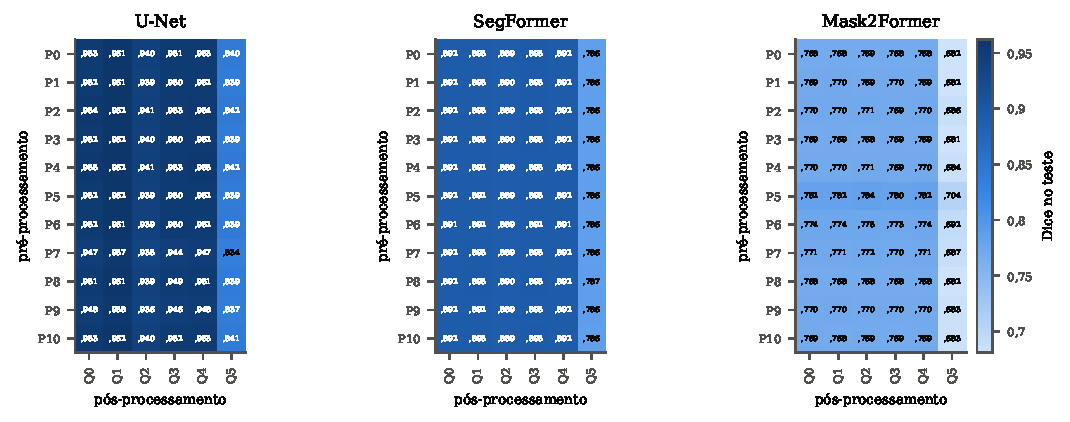
\includegraphics[width=0.82\textwidth]{heatmap_dice}
\caption{Dice no teste de todas as combinações de pré-processamento (linhas) e pós-processamento (colunas) para cada arquitetura. P0 e Q0 indicam os \textit{baselines}.}
\label{fig:heat}
\end{figure*}

A configuração de maior Dice de validação entre as 198 combinações, a U-Net com normalização RMS e otimização do limiar (E006), é apresentada na Tabela~\ref{tab:best_configuration}, e a Tabela~\ref{tab:cross_dataset} traz a linha deste conjunto no resumo entre conjuntos. Seu ganho relativo de 0,95\% sobre a U-Net sozinha depende do instante inicial, como examinado na Seção~\ref{subsec:sensitivity}.

\begin{table*}[t]
\centering
\caption{Melhor configuração escolhida na validação e desempenho no teste. Critério de seleção fixado antes do teste: maior Dice médio de validação entre as 198 combinações.}
\label{tab:best_configuration}
\small
\begin{tabularx}{\textwidth}{L{4.3cm} L{1.6cm} L{2.4cm} L{2.8cm} c c c}
\toprule
\textbf{Conjunto} & \textbf{Arquitetura} & \textbf{Pré-processamento} & \textbf{Pós-processamento} & \textbf{IoU} & \textbf{Dice} & \textbf{IC 95\% (Dice)} \\
\midrule
\texttt{gray\_scott\_reaction\_}\newline\texttt{diffusion} & U-Net & P2 RMS & Q1 Otimização do limiar & 0,950 & 0,962 & [0,960; 0,964] \\
\bottomrule
\end{tabularx}
\vspace{6pt}
\caption{Resumo entre conjuntos da abordagem de segmentação escolhida. Ganho relativo: Dice no teste da configuração escolhida em relação à mesma arquitetura sem pré e pós-processamento.}
\label{tab:cross_dataset}
\small
\begin{tabularx}{\textwidth}{L{4.3cm} L{1.7cm} L{1.4cm} c c Y}
\toprule
\textbf{Conjunto} & \textbf{Arquitetura escolhida} & \textbf{P / Q escolhidos} & \textbf{Dice no teste} & \textbf{Ganho relativo (\%)} & \textbf{Observações de generalização} \\
\midrule
\texttt{gray\_scott\_reaction\_}\newline\texttt{diffusion} & U-Net & P2 / Q1 & 0,962 & +0,95 & O ganho sobre a U-Net sozinha (0,953) vem do instante inicial aleatório; em $n\geq50$, Dice de 0,992 contra 0,995 ($-$0,2\%). \\
\bottomrule
\end{tabularx}
\end{table*}


\subsection{Apresentação estatística}\label{subsec:statistics}

Todos os valores são médias sobre as 120 trajetórias de teste, a unidade estatística, com intervalos por \textit{bootstrap} estratificado (Seção~\ref{subsec:cost}); quadros adjacentes de uma mesma trajetória não são tratados como observações independentes. Com uma semente por configuração, os intervalos capturam a variação entre trajetórias de teste, mas não entre treinos. O teste não foi usado para escolher limiares, parâmetros de pós-processamento ou hiperparâmetros.

A Tabela~\ref{tab:classwise_temporal} mostra um aspecto que o Dice da classe estrutura não revela. Na U-Net, a otimização do limiar elevou o Dice da estrutura, mas reduziu o IoU da classe fundo de 0,986 para 0,952 e o mIoU de 0,967 para 0,950; no SegFormer, o IoU do fundo caiu de 0,928 para 0,872, e o IoU da estrutura caiu 1,18 ponto (Tabela~\ref{tab:prepost_effect}), enquanto seu Dice não se alterou. A troca decorre do limiar escolhido na validação, 0,2 para a U-Net e para o SegFormer, que amplia a região classificada como estrutura.

\begin{table*}[t]
\centering
\caption{Métricas por classe e temporais no teste para as configurações da Tabela~\ref{tab:full_results}. IoU$_{f}$, Dice$_{f}$: classe fundo; mIoU: média do IoU das duas classes; AVE: erro de variação de área (\% do domínio por instante amostrado); CDE: erro de deslocamento dos centroides das estruturas (pixels, distância periódica); TC: consistência temporal das máscaras; TCE $=|\mathrm{TC}_{pred}-\mathrm{TC}_{GT}|$; memória: pico de memória da GPU na inferência (lote 1). Média $\pm$ meia-amplitude do IC de 95\%.}
\label{tab:classwise_temporal}
\scriptsize
\setlength{\tabcolsep}{3pt}
\begin{tabularx}{\textwidth}{L{0.7cm} L{1.6cm} Y c c c c c c c c}
\toprule
\textbf{ID} & \textbf{Arquitetura} & \textbf{Condição} & \textbf{IoU$_{f}$} & \textbf{Dice$_{f}$} & \textbf{mIoU} & \textbf{AVE (\%)} & \textbf{CDE (px)} & \textbf{TC} & \textbf{TCE} & \textbf{Mem. (MiB)} \\
\midrule
E151 & U-Net & Arquitetura sozinha (P0+Q0) & 0,986{\scriptsize$\pm$0,001} & 0,992{\scriptsize$\pm$0,001} & 0,967{\scriptsize$\pm$0,001} & 0,76{\scriptsize$\pm$0,05} & 2,68{\scriptsize$\pm$0,34} & 0,686 & 0,010{\scriptsize$\pm$0,002} & 170 \\
E160 & U-Net & Pré + arq. (P4+Q0) & 0,986{\scriptsize$\pm$0,001} & 0,992{\scriptsize$\pm$0,001} & 0,967{\scriptsize$\pm$0,001} & 0,59{\scriptsize$\pm$0,07} & 2,16{\scriptsize$\pm$0,34} & 0,683 & 0,007{\scriptsize$\pm$0,001} & 170 \\
E152 & U-Net & Arq. + pós (P0+Q1) & 0,952{\scriptsize$\pm$0,002} & 0,957{\scriptsize$\pm$0,002} & 0,950{\scriptsize$\pm$0,002} & 3,55{\scriptsize$\pm$0,14} & 1,57{\scriptsize$\pm$0,22} & 0,691 & 0,009{\scriptsize$\pm$0,001} & 170 \\
E006 & U-Net & Pré + arq. + pós (P2+Q1) & 0,952{\scriptsize$\pm$0,002} & 0,957{\scriptsize$\pm$0,002} & 0,951{\scriptsize$\pm$0,002} & 3,58{\scriptsize$\pm$0,15} & 1,42{\scriptsize$\pm$0,21} & 0,691 & 0,008{\scriptsize$\pm$0,001} & 170 \\
\addlinespace
E167 & SegFormer & Arquitetura sozinha (P0+Q0) & 0,928{\scriptsize$\pm$0,002} & 0,961{\scriptsize$\pm$0,001} & 0,883{\scriptsize$\pm$0,003} & 0,89{\scriptsize$\pm$0,05} & 7,16{\scriptsize$\pm$0,69} & 0,685 & 0,013{\scriptsize$\pm$0,002} & 227 \\
E180 & SegFormer & Pré + arq. (P8+Q0) & 0,929{\scriptsize$\pm$0,002} & 0,962{\scriptsize$\pm$0,001} & 0,883{\scriptsize$\pm$0,003} & 0,89{\scriptsize$\pm$0,05} & 7,18{\scriptsize$\pm$0,67} & 0,685 & 0,013{\scriptsize$\pm$0,002} & 227 \\
E168 & SegFormer & Arq. + pós (P0+Q1) & 0,872{\scriptsize$\pm$0,002} & 0,912{\scriptsize$\pm$0,002} & 0,849{\scriptsize$\pm$0,003} & 3,87{\scriptsize$\pm$0,15} & 7,85{\scriptsize$\pm$0,62} & 0,698 & 0,014{\scriptsize$\pm$0,001} & 227 \\
E086 & SegFormer & Pré + arq. + pós (P8+Q1) & 0,873{\scriptsize$\pm$0,002} & 0,912{\scriptsize$\pm$0,002} & 0,850{\scriptsize$\pm$0,003} & 3,87{\scriptsize$\pm$0,15} & 7,91{\scriptsize$\pm$0,60} & 0,697 & 0,014{\scriptsize$\pm$0,001} & 227 \\
\addlinespace
E183 & Mask2Former & Arquitetura sozinha (P0+Q0) & 0,836{\scriptsize$\pm$0,007} & 0,908{\scriptsize$\pm$0,004} & 0,742{\scriptsize$\pm$0,008} & 1,20{\scriptsize$\pm$0,05} & 9,47{\scriptsize$\pm$0,64} & 0,686 & 0,014{\scriptsize$\pm$0,002} & 287 \\
E193 & Mask2Former & Pré + arq. (P5+Q0) & 0,796{\scriptsize$\pm$0,006} & 0,866{\scriptsize$\pm$0,003} & 0,727{\scriptsize$\pm$0,008} & 4,08{\scriptsize$\pm$0,14} & 7,13{\scriptsize$\pm$0,65} & 0,697 & 0,012{\scriptsize$\pm$0,001} & 287 \\
E185 & Mask2Former & Arq. + pós (P0+Q2) & 0,839{\scriptsize$\pm$0,007} & 0,910{\scriptsize$\pm$0,004} & 0,744{\scriptsize$\pm$0,008} & 1,20{\scriptsize$\pm$0,05} & 9,95{\scriptsize$\pm$0,76} & 0,684 & 0,015{\scriptsize$\pm$0,002} & 287 \\
E122 & Mask2Former & Pré + arq. + pós (P5+Q2) & 0,800{\scriptsize$\pm$0,006} & 0,869{\scriptsize$\pm$0,003} & 0,730{\scriptsize$\pm$0,008} & 4,10{\scriptsize$\pm$0,14} & 7,45{\scriptsize$\pm$0,81} & 0,695 & 0,010{\scriptsize$\pm$0,001} & 287 \\
\addlinespace
REF & Otsu em $A$ & Referência (P0+Q0) & 0,916{\scriptsize$\pm$0,005} & 0,951{\scriptsize$\pm$0,003} & 0,871{\scriptsize$\pm$0,008} & 1,76{\scriptsize$\pm$0,13} & 3,17{\scriptsize$\pm$0,43} & 0,710 & 0,027{\scriptsize$\pm$0,003} & n/d \\
\bottomrule
\end{tabularx}
\end{table*}


\subsection{Tabelas visuais e evolução temporal}\label{subsec:visual}

As Figuras~\ref{fig:vt_spirals} e~\ref{fig:vt_gliders} apresentam, para uma trajetória de teste de dois regimes, o instante inicial ($n=0$), dois instantes intermediários e o instante final ($n=1000$). O instante $n=50$ é o primeiro amostrado após a condição inicial e registra a organização do padrão, e $n=500$ é o quadro característico sobre o qual a referência foi definida. Para cada arquitetura, as figuras mostram a entrada $A$, a entrada após o pré-processamento escolhido, a referência e as máscaras das quatro condições. Em $n=0$, as arquiteturas sem pós-processamento erram a maior parte da referência, com predomínio de falsos negativos, enquanto as configurações com limiar reduzido e o Mask2Former com recorte por percentis segmentam quase todo o domínio, com predomínio de falsos positivos. A partir de $n=50$, a U-Net acompanha as estruturas com poucos erros, enquanto o SegFormer e o Mask2Former concentram erros nas fronteiras.

\begin{figure*}[t]
\centering
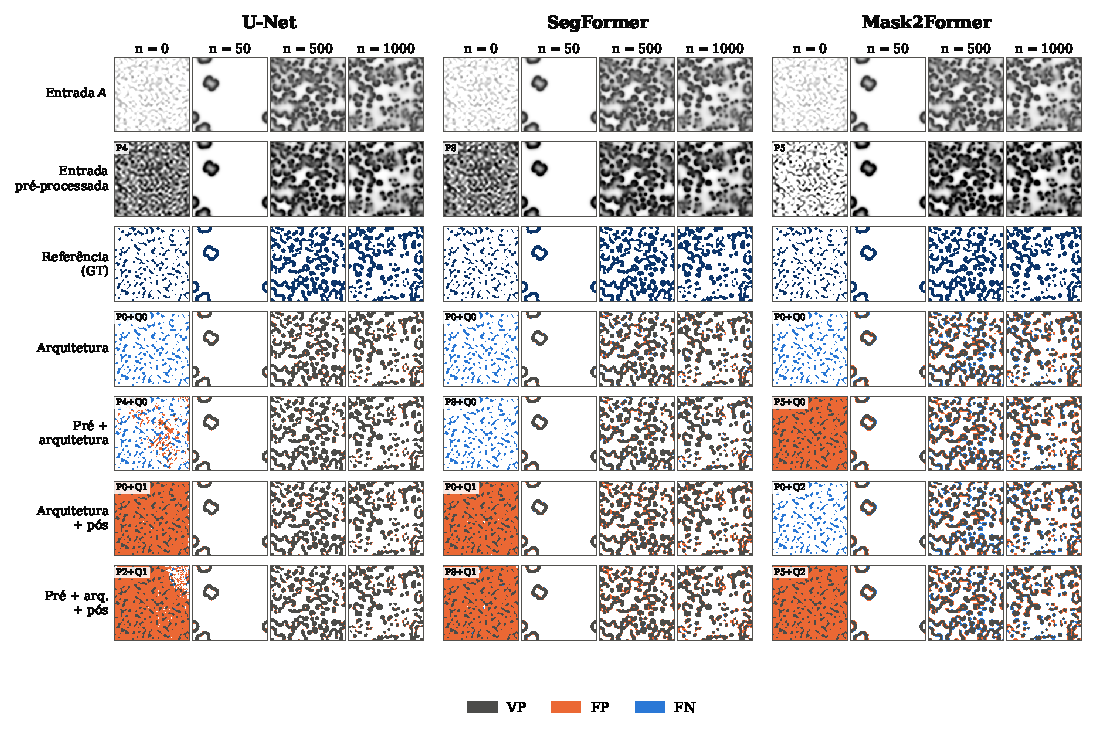
\includegraphics[width=0.84\textwidth]{visual_table_spirals}
\caption{Tabela visual do regime \textit{spirals}. Para cada arquitetura: entrada $A$, entrada pré-processada, referência e máscaras das quatro condições em $n=0$, $50$, $500$ e $1000$. Cinza-escuro: verdadeiro positivo; laranja: falso positivo; azul: falso negativo.}
\label{fig:vt_spirals}
\end{figure*}

\begin{figure*}[t]
\centering
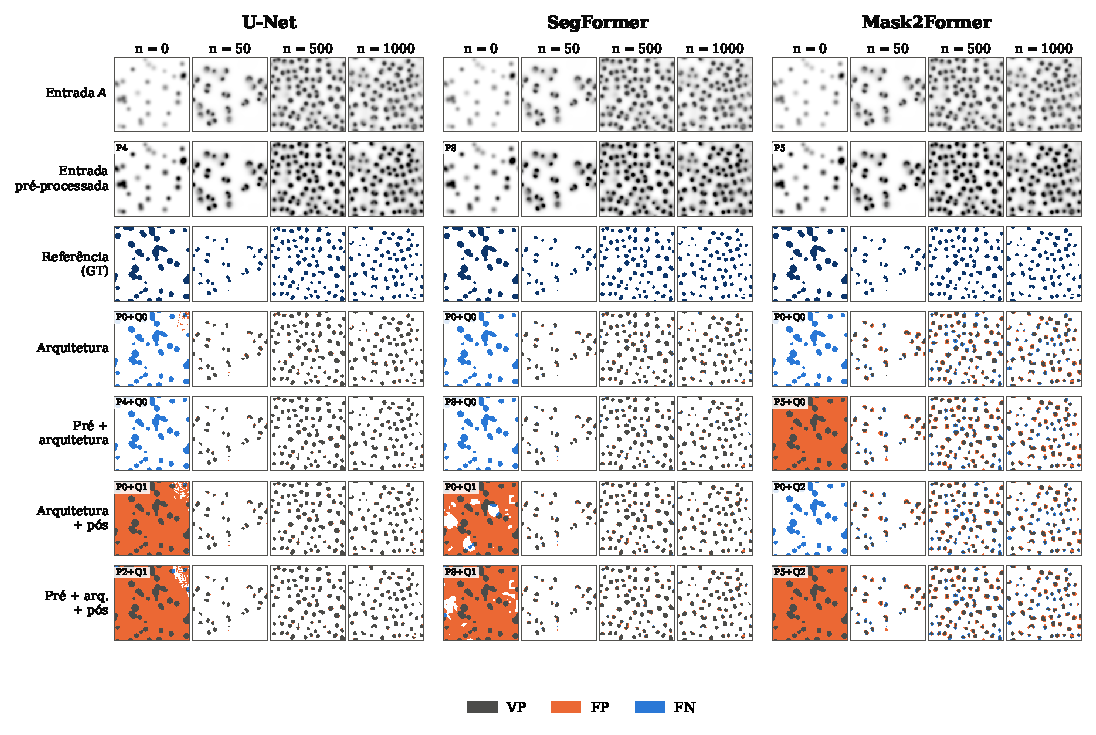
\includegraphics[width=0.84\textwidth]{visual_table_gliders}
\caption{Tabela visual do regime \textit{gliders}, com manchas que se deslocam e se dividem. Mesma organização da Figura~\ref{fig:vt_spirals}.}
\label{fig:vt_gliders}
\end{figure*}

Em $n=50$, a U-Net sozinha já alcançava Dice de 0,994, o SegFormer, 0,952 e o Mask2Former, 0,829, e a partir de $n=100$ as médias foram de 0,995, 0,930 e 0,800 (Figura~\ref{fig:temporal}); a referência obteve 0,869 em $n=50$ e 0,923 a partir de $n=100$. A U-Net sozinha teve o menor erro de variação de área, 0,76\% do domínio por instante amostrado, e TCE de 0,010, para uma consistência temporal de 0,689 na referência (Tabela~\ref{tab:classwise_temporal}). Sua configuração final (P2+Q1) reduziu o erro de centroide de 2,68 para 1,42 pixel, mas elevou o erro de variação de área para 3,58\%, efeito do salto de área entre o instante inicial supersegmentado e os seguintes. O SegFormer e o Mask2Former mantiveram erros de centroide de 7,1 a 10,0 pixels. A U-Net acompanhou, portanto, a evolução das estruturas a partir do primeiro instante amostrado após a condição inicial, enquanto nenhuma configuração segmentou o instante inicial de forma informativa (PP4).

\begin{figure}[t]
\centering
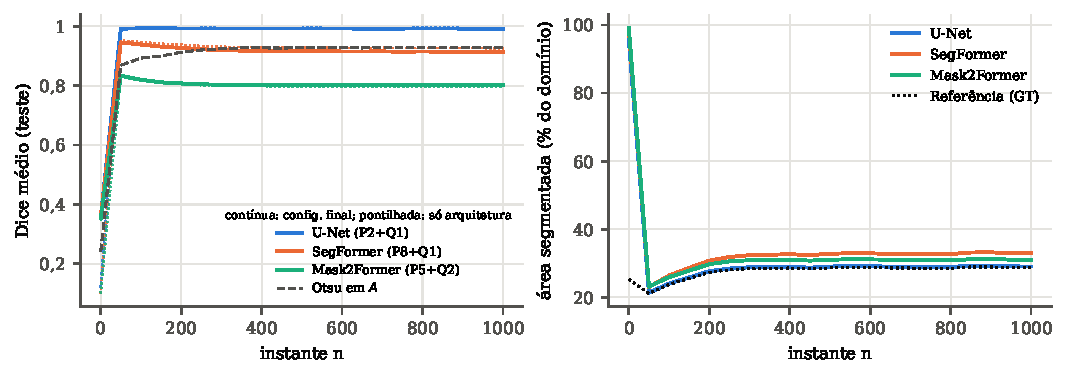
\includegraphics[width=\columnwidth]{temporal_dice_area}
\caption{À esquerda, Dice médio no teste por instante para a configuração final de cada arquitetura (contínua), para a arquitetura sozinha (pontilhada) e para Otsu em $A$ (tracejada). À direita, área segmentada média (\% do domínio).}
\label{fig:temporal}
\end{figure}

\subsection{Sensibilidade ao instante inicial}\label{subsec:sensitivity}

O instante $n=0$ é um dos 21 instantes amostrados, e nele a condição inicial é aleatória. A Tabela~\ref{tab:sensitivity} separa o Dice desse instante do Dice dos demais. As arquiteturas sem pós-processamento obtiveram Dice entre 0,100 e 0,120 em $n=0$, com a U-Net prevendo cerca de 11\% do domínio, contra 25,3\% da referência. Com o limiar de 0,2, a U-Net passou a segmentar 95,2\% do domínio nesse instante, e seu Dice subiu para 0,353. Nos instantes $n\geq50$, contudo, a configuração P2+Q1 obteve 0,992, abaixo dos 0,995 da U-Net sozinha. Recalculado sem o instante inicial, o efeito pareado da otimização do limiar mudou de sinal: $-0,28$ ponto na U-Net e $-1,21$ no SegFormer, ambos distinguíveis de zero (Tabela~\ref{tab:prepost_effect}). O efeito do recorte por percentis no Mask2Former caiu de 1,37 para 0,18 ponto, pois essa configuração também previu 99,2\% do domínio em $n=0$. Os efeitos da abertura e do filtro temporal mantiveram o sinal e a magnitude. Sem o instante inicial, o SegFormer obteve 0,931, acima dos 0,921 da referência.

\begin{table}[t]
\centering
\caption{Sensibilidade ao instante inicial: Dice médio no teste nos 21 instantes, apenas no instante inicial aleatório $n=0$ e nos 20 instantes $n\geq50$.}
\label{tab:sensitivity}
\scriptsize
\setlength{\tabcolsep}{3pt}
\begin{tabularx}{\columnwidth}{L{0.7cm} Y c c c}
\toprule
\textbf{ID} & \textbf{Configuração} & \textbf{Todos} & \textbf{$n=0$} & \textbf{$n\geq50$} \\
\midrule
E151 & U-Net (P0+Q0) & 0,953 & 0,120 & 0,995 \\
E160 & U-Net (P4+Q0) & 0,955 & 0,153 & 0,995 \\
E152 & U-Net (P0+Q1) & 0,961 & 0,353 & 0,992 \\
E006 & U-Net (P2+Q1) & 0,962 & 0,354 & 0,992 \\
\addlinespace
E167 & SegFormer (P0+Q0) & 0,892 & 0,100 & 0,931 \\
E180 & SegFormer (P8+Q0) & 0,892 & 0,100 & 0,932 \\
E168 & SegFormer (P0+Q1) & 0,893 & 0,357 & 0,919 \\
E086 & SegFormer (P8+Q1) & 0,893 & 0,357 & 0,920 \\
\addlinespace
E183 & Mask2Former (P0+Q0) & 0,768 & 0,102 & 0,801 \\
E193 & Mask2Former (P5+Q0) & 0,782 & 0,353 & 0,803 \\
E185 & Mask2Former (P0+Q2) & 0,769 & 0,101 & 0,802 \\
E122 & Mask2Former (P5+Q2) & 0,784 & 0,353 & 0,805 \\
\addlinespace
REF & Otsu em $A$ (P0+Q0) & 0,888 & 0,241 & 0,921 \\
\bottomrule
\end{tabularx}
\end{table}


\subsection{Regimes de padrão e custo computacional}\label{subsec:regimes}

A U-Net sozinha manteve Dice entre 0,943 e 0,979 em todos os regimes (Tabela~\ref{tab:regime}). O SegFormer obteve seus menores valores em \textit{spots} (0,833), \textit{maze} (0,865) e \textit{worms} (0,868), abaixo dos 0,906, 0,938 e 0,896 da referência nesses regimes, que são os de menor comprimento de onda (Tabela~\ref{tab:regimes}); o Mask2Former também obteve seu menor valor em \textit{spots} (0,667).

\begin{table}[t]
\centering
\caption{Dice no teste por regime de padrão (20 trajetórias de teste cada) para cada arquitetura sozinha, para seu par de pré e pós-processamento escolhido na validação e para a referência sem aprendizado.}
\label{tab:regime}
\scriptsize
\setlength{\tabcolsep}{2.5pt}
\begin{tabularx}{\columnwidth}{Y *{6}{c}}
\toprule
\textbf{Configuração} & \textbf{Glid.} & \textbf{Bubb.} & \textbf{Maze} & \textbf{Worms} & \textbf{Spir.} & \textbf{Spots} \\
\midrule
U-Net (P0+Q0) & 0,948 & 0,979 & 0,950 & 0,948 & 0,943 & 0,949 \\
U-Net (P2+Q1) & 0,963 & 0,981 & 0,959 & 0,956 & 0,955 & 0,958 \\
SegFormer (P0+Q0) & 0,927 & 0,952 & 0,865 & 0,868 & 0,905 & 0,833 \\
SegFormer (P8+Q1) & 0,941 & 0,952 & 0,859 & 0,866 & 0,912 & 0,829 \\
Mask2Former (P0+Q0) & 0,833 & 0,800 & 0,781 & 0,712 & 0,816 & 0,667 \\
Mask2Former (P5+Q2) & 0,850 & 0,803 & 0,795 & 0,726 & 0,835 & 0,692 \\
Otsu em $A$ (P0+Q0) & 0,852 & 0,917 & 0,938 & 0,896 & 0,821 & 0,906 \\
\bottomrule
\end{tabularx}
\end{table}

\begin{table}[t]
\centering
\caption{Tamanho e custo dos modelos (20 épocas, lote 32, entrada nativa de $128\times128$, entrada de referência P0). Melhor época: época do ponto de verificação com maior Dice de validação, intervalo entre as 11 entradas P0 a P10. Latência e vazão medidas com a GPU dedicada após todos os treinos.}
\label{tab:cost}
\scriptsize
\setlength{\tabcolsep}{3pt}
\begin{tabularx}{\columnwidth}{Y c c c c c}
\toprule
\textbf{Arquitetura} & \textbf{Parâm. (M)} & \textbf{Treino (min)} & \textbf{Melhor época} & \textbf{Latência (ms)} & \textbf{qps} \\
\midrule
U-Net & 24,4 & 21 & 11 a 20 & 5,58 & 4932 \\
SegFormer & 27,3 & 35 & 19 a 20 & 15,61 & 2073 \\
Mask2Former & 47,4 & 273 & 1 a 9 & 38,63 & 552 \\
\bottomrule
\end{tabularx}
\end{table}


A U-Net teve a menor latência (5,58~ms) e o menor tempo de treino, enquanto o Mask2Former, com 47,4 milhões de parâmetros, teve latência de 38,63~ms e o maior tempo de treino na execução compartilhada (Tabela~\ref{tab:cost}). A época escolhida também diferiu: no SegFormer, foi a época 19 ou 20 em todas as entradas, o que indica que seu Dice de validação ainda crescia ao fim do orçamento; no Mask2Former, ficou entre as épocas 1 e 9, pois seu Dice de validação permaneceu entre 0,771 e 0,776 ao longo das 20 épocas na entrada de referência.

%% ============================================================================
\section{Discussão, aplicabilidade e limitações}\label{sec:sec6}

\subsection{Arquiteturas e resolução de saída}\label{subsec:disc_arch}

A ordem entre as arquiteturas foi determinada por uma propriedade de projeto, a resolução de saída, mais do que pelas técnicas aplicadas antes ou depois da rede. A U-Net prevê na resolução da entrada, com conexões de salto a partir do estágio de maior resolução, ao passo que o SegFormer e o Mask2Former preveem em $32\times32$ células para uma entrada de $128\times128$. Com estruturas de poucos pixels de diâmetro (Tabela~\ref{tab:regimes}), uma célula da saída dessas arquiteturas cobre parte considerável de uma estrutura, e a fronteira passa a depender da interpolação dos \textit{logits}. Essa interpretação é compatível com a queda do SegFormer nos regimes de menor comprimento de onda, nos quais ficou abaixo da limiarização de $A$. O desenho, contudo, não isola a resolução de saída de outras diferenças entre as arquiteturas, como o \textit{backbone} e o pré-treinamento.

O desempenho do Mask2Former deve ser lido com cautela. Seu Dice de validação estabilizou-se nas primeiras épocas, enquanto a perda de treino continuava diminuindo, o que é compatível com duas hipóteses não separadas pelo desenho: a saída em baixa resolução e o treino sem supervisão profunda~\cite{cheng2022mask2former}. Seus resultados caracterizam, assim, a configuração efetivamente treinada, e não o potencial da arquitetura. No SegFormer, a melhor época ao fim do orçamento indica que o limite de 20 épocas pode tê-lo restringido.

\subsection{Por que o pré e o pós-processamento melhoraram ou pioraram}\label{subsec:disc_why}

O efeito pequeno do pré-processamento é compatível com as propriedades dos dados. Os campos simulados não contêm ruído de aquisição, de modo que os filtros de remoção de ruído têm pouco a remover, enquanto os filtros de suavização removem sinal: a suavização gaussiana atenua os harmônicos que definem fronteiras nítidas, e o filtro de mediana arredonda cantos e remove ligações de um pixel. Essa perda de detalhe é compatível com as reduções observadas na U-Net, a única arquitetura capaz de explorar esse detalhe. As normalizações são, em primeira ordem, transformações afins cujo efeito tende a ser absorvido pelas camadas de normalização das redes, o que é coerente com efeitos próximos de zero.

Os efeitos do pós-processamento acompanharam a escala das operações em relação às estruturas e à amostragem temporal. A abertura com disco de raio 1 remove estruturas com menos de três pixels de largura, como as manchas nascentes e as paredes finas do regime \textit{bubbles}, que a U-Net já preservava. A ausência de efeito da filtragem de componentes conexos é compatível com o fato de que redes aplicadas a campos suaves quase não produzem regiões isoladas de poucos pixels, de modo que a hipótese de ruído pontual que justifica o método não se verificou neste conjunto. O filtro temporal combina instantes separados por 500 unidades de tempo; onde o padrão se desloca, as estruturas mudam de posição nesse intervalo, e a mediana produz máscaras defasadas que apagam mudanças físicas reais, o que é coerente com perdas de cerca de 30 pontos em \textit{gliders} e \textit{spirals} e com a ressalva do próprio protocolo sobre esse método.

\subsection{Critério de seleção e instante inicial}\label{subsec:disc_n0}

A sensibilidade ao instante inicial é o resultado de maior consequência metodológica. Em $n=0$, a condição inicial é aleatória, e $A$ ainda não reflete a estrutura de $B$, de modo que nenhuma configuração segmentou esse instante de forma informativa. Ainda assim, um único instante entre 21 bastou para decidir a seleção na validação: um limiar baixo leva a rede a segmentar quase todo o domínio em $n=0$, o que aumenta o Dice desse quadro sem nenhuma informação física, e o mesmo efeito explica a maior parte do ganho do recorte por percentis no Mask2Former. Nos instantes com padrão, a otimização do limiar reduziu o Dice da U-Net e do SegFormer e reduziu o IoU da classe fundo, o que mostra que o Dice médio da classe estrutura, usado como critério único de seleção, favoreceu a supersegmentação de um quadro sem informação. A escolha de uma configuração para acompanhar a evolução das estruturas deve, portanto, considerar as métricas por classe e as temporais e excluir ou ponderar o instante inicial quando a condição inicial é aleatória. Outros conjuntos da turma com condições iniciais aleatórias ou sem estrutura podem estar sujeitos ao mesmo efeito quando seus resultados forem reunidos.

\subsection{Aplicabilidade e viabilidade em tempo real}\label{subsec:disc_realtime}

Com 5,58~ms por quadro de $128\times128$, a U-Net segmenta cerca de 180 quadros por segundo com lote 1 e cerca de 4.900 em lotes, de modo que uma trajetória de 1.001 instantes leva menos de um segundo, custo compatível com o monitoramento de uma simulação ou de um substituto neural durante sua execução. A referência sem aprendizado é cerca de 18 vezes mais rápida (0,30~ms), mas perde 6,5 pontos de Dice em todos os instantes e 7,4 nos instantes com padrão; o pós-processamento acrescentou no máximo 0,51~ms por quadro, em uma GPU e com lote 1.

\subsection{Limitações}\label{subsec:limitations}

Quanto à validade interna, cada configuração foi treinada com uma única semente, o Mask2Former sem supervisão profunda, e as arquiteturas diferem simultaneamente em resolução de saída, \textit{backbone} e pré-treinamento, de modo que nenhuma comparação entre elas identifica a causa das diferenças; os treinos também compartilharam a GPU, o que afeta os tempos de treino, mas não as latências. Quanto à validade de construção, a referência foi definida por limiarização de $B$, e não por anotação especialista, e depende do instante de referência e do critério de Otsu, de modo que o experimento mede a recuperação de uma segmentação definida por critério físico; a anticorrelação entre $A$ e $B$ torna a tarefa mais simples que a segmentação de imagens naturais, razão pela qual a referência sem aprendizado foi incluída; e o intervalo de 50 instantes limita a resolução temporal das métricas de evolução. Quanto à validade externa, os resultados referem-se a um sistema físico, a uma GPU e a redes que processam quadros isolados.

%% ============================================================================
\section{Conclusão}\label{sec:conclusions}

Este trabalho avaliou o pré-processamento, a arquitetura e o pós-processamento na segmentação temporal das regiões de reação ativa no sistema de Gray-Scott do The Well, sob o protocolo comum da turma. A U-Net obteve Dice de 0,953 sem pré e pós-processamento, acima da referência de Otsu em $A$ (0,888), enquanto o SegFormer não se distinguiu dessa referência (0,892) e o Mask2Former ficou abaixo dela (0,768). O pré-processamento alterou o Dice em no máximo 1,37 ponto percentual, e o maior efeito decorreu do instante inicial. A otimização do limiar elevou o Dice médio da U-Net em 0,84 ponto, mas passou a reduzi-lo quando o instante inicial foi excluído, e a filtragem de consistência temporal reduziu o Dice de todas as arquiteturas em 8,6 a 11,3 pontos, com perdas de cerca de 30 pontos nos regimes cujas estruturas se deslocam. A U-Net acompanhou a evolução das estruturas a partir do primeiro instante amostrado, com Dice médio de 0,995 a partir de $n=100$, mas nenhuma configuração segmentou o instante inicial aleatório. Nesse conjunto, a resolução de saída da arquitetura pesou mais que as técnicas aplicadas antes e depois dela, e a seleção de configurações pelo Dice médio mostrou-se sensível a um único quadro sem informação física.

A continuidade do estudo requer mais sementes, o Mask2Former com supervisão profunda, arquiteturas Transformer com resolução de saída variada, um critério de seleção que exclua ou pondere o instante inicial, arquiteturas com contexto temporal e a integração destes resultados aos dos demais conjuntos da turma.

%% ============================================================================
%% SECOES FINAIS OBRIGATORIAS (BACKMATTER)
%% ============================================================================
\section*{Declaração de contribuição de autoria (CRediT)}
%% Papeis CRediT de cada autor: confirmar com os autores antes da entrega.
\textbf{Andre Luis Aguiar do Nascimento:} [papéis a definir].
\textbf{Joao Guilherme Miranda Lago:} [papéis a definir].
\textbf{Wesley dos Santos Gatinho:} Conceitualização, Metodologia, Software, Investigação, Análise formal, Curadoria de dados, Visualização, Escrita (rascunho original), Escrita (revisão e edição).

\section*{Declaração de conflito de interesses}
Os autores declaram não ter interesses financeiros concorrentes ou relações pessoais conhecidas que possam ter influenciado o trabalho relatado neste artigo.

\section*{Disponibilidade de dados}
Os dados estão disponíveis publicamente no The Well (\url{https://polymathic-ai.org/the_well/}). Os identificadores das trajetórias, os resultados por combinação (\texttt{results\_sequential.csv}, \texttt{results\_protocolo.csv}) e o código que obtém o subconjunto, constrói a referência, treina os modelos e gera todas as tabelas e figuras estão disponíveis com os autores.

%% ============================================================================
%% REFERENCIAS (estilo numerico Elsevier: elsarticle-num)
%% ============================================================================
\setlength{\bibsep}{1pt plus 0.5pt}
\renewcommand{\bibfont}{\footnotesize}
\bibliographystyle{elsarticle-num}
\bibliography{references}

\end{document}
